\chapter{实数}
实数是现实世界中最基本的数系,我们采用逼近法来研
究实数,逼近法是一种原理简朴但是应用广泛的方法,它将
贯穿于本书的微积分学部分,是一支主力军。

\section{度量与实数}

一般说来,常见的量可以归纳成两类:比如一堆蛋,
一群牛,它们都具有天然的个别单元,对它们的处理方法是
数一数它们的个数,用来数个数的数学体系就是“自然数系”。
另一类量如长度、重量、温度、压力这种量不具有天然不可
分割的单元!我们处理这类量的办法是度量,由度量产生的
数系就是“实数系”,换句话说,实数系乃是将常见的长度、
重量等这一类量的通性加以抽象化、组织化所得出来的数学
体系,它是用来表达、计算这一类连续变化的量的简洁、有
效工具。

下面将以长度为例,说明度量和实数的起源。

\subsection{长度的度量}
因为长度这种量并不是有天然不可分割的单位,所以我
们只好选用人为的单位长,设线段
$u$是所选用的单位长,当
我们要度量一个线段$a$时,我们所要去求的乃是$a$与$u$之间的
“比值”,这个比值是一个实数$k$, 我们就说线段$a$的长度是
$k$单位,现在让我们耐心地分析一下,在实践中这个“比
值”是怎样求得的?

我们先拿一根尺$u$, 用它 
去逐段比量线段$a$, 假如$a$恰好是$n$个和$u$等长的线段首尾连接
而成,我们说$u$恰好整量$a$, $a$的长度是$n$单位,但是假如$u$
不能整量$a$,例如在图6.1中的线段,$a$比$4u$要长些,却比$5u$要
短些。

\begin{figure}[htp]
    \centering
\begin{tikzpicture}
\draw (0,1)--node[above]{$u$}(1,1);
\foreach \x in {0,1}
{
    \draw (\x,1)--(\x,1.1);
}
\draw (0,0)--node[above=5pt]{$a$}(4.75,0);
\foreach \x in {0,1,...,4,4.25,4.5,4.75}
{
    \draw (\x,0)--(\x,0.1);
}
\end{tikzpicture}
    \caption{}
\end{figure}


试着去解决上述不能整量的矛盾的一个简朴想法是:把
单位长$u$适当地加以等分,希望分后的“分单位”能够整量
$a$(比如上面的例子中,$\frac{1}{4}u$
就可以整量$a$, 即$a=4\frac{3}{4}u=\frac{19}{4}u$),一般地,假如$a$
能用$\frac{1}{m}u$这个分单位整量,譬如$a=\frac{n}{m}u$,则$a,u$之间的比值是个有理数(也称为比数)。在
这儿,就自然地产生下述基本问题。

\textbf{度量基本问题 } 任给两个量$a,b$之间的比值是否一定是
个有理数(比数)?换句话说,对于任给两个量$a,b$是否存
在一个同时整量$a,b$的$u$?

上面这个问题的重要性可以分别从正、反两面来分析:
假如任何两个量的比值总是有理数,那么有理数全体就足够
处理度量问题,这样度量问题就变得十分简单了。从另一方
面来看,假如两个量之间的比值不一定是有理数,则有理数
全体(简称有理数系或比数系)就不足以处理度量问题,换
句话说,我们就得学会一个不只包含有理数系的实数系,才
能充分处理度量问题。总之,上述基本问题是必须实事求是
地弄明白的!

\subsection{无理数(非比实数)的存在}
不难给出,两个线段的比值不可能是有理数的一个简单
例子,如图6.2所示,各边为单位长
度的正方形的对角线$\ell$与边长之比就
不能是个有理数。
\begin{figure}[htp]
    \centering
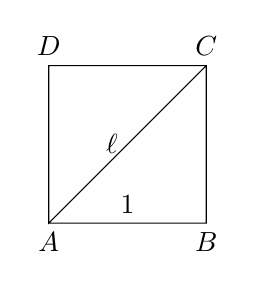
\begin{tikzpicture}
\draw (0,0)node[below]{$A$} --node[above]{1}(2,0)node[below]{$B$}-- (2,2)node[above]{$C$}--(0,2)node[above]{$D$}--(0,0)--node[left]{$\ell$}(2,2);
\end{tikzpicture}
    \caption{}
\end{figure}

因为根据勾股定理,
$\ell^2=2$, 所以,如果$\ell$是个有理数,设其等于
$\frac{p}{q}$,这里$q$和$p$是两个互质的正整
数,我们将有
\[p^2=2q^2\]
根据上述方程,$p$是偶数,因此$p$本身也必定是偶数,譬如
说,$p=2p'$, 用$2p'$代替$p$, 我们得到
\[4({p'}^2)=2q^2\]
或者,
\[q^2=2(p')^2\]
因而$q^2$是偶数,于是$q$也是偶数,然而这同我们所作的$p$和$q$没
有公因子的约定相矛盾,这一矛盾是由假设对角线长能够表
示为既约分数$\frac{p}{q}$
引起的,所以这一假设是错误的。

这一用反证法推导的例子,表明符号$\sqrt{2}$不能对应于任
何有理数。另一例子是$\pi$——圆的周长与直径的比,证明$\pi$
不是有理数要复杂得多,并且直到近代才做到。不属于有理
数系的实数有很多,所以在某种意义上远比有理数更为普
遍,因此,从几何度量的客观实际需要出发,我们不得不增
添一类新数,这一类新数叫\textbf{无理数}。有理数和无理数的全体
统称为\textbf{实数系}。当我们面对着实数系中还存在着许多“无理
数”这一事实时,怎样去有系统地学习实数系的性质并充分
掌握其用法,这便成为我们的一个迫切的基本课题。下面所
要谈的逼近法,就是一种有效地利用熟知的有理数系作为桥
梁,向实数系进军的捷径。

\subsection{逼近法}
通过已知的有理数系去了解实数系的可能性基于下述基
本事实,那就是:任何无理数都可以用有理数去逼近它!
现在我们用数轴来图解有理数系与实数系间的关系。如图6.3
所示。

\begin{figure}[htp]
    \centering
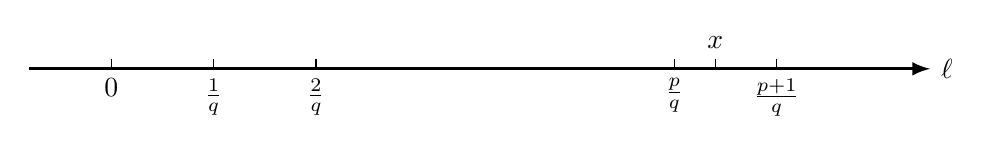
\begin{tikzpicture}[>=latex, scale=1.3]
\draw[very thick, ->] (-0.8,0)--(8,0)node[right]{$\ell$};
\foreach \x/\xtext in {0/0,1/\frac{1}{q},2/\frac{2}{q},5.5/\frac{p}{q},6.5/\frac{p+1}{q}}
{
    \draw (\x, 0)node[below]{$\xtext$}--(\x,.1);
} 
\draw (5.9,0)--(5.9,.1)node[above]{$x$};

\end{tikzpicture}
    \caption{}
\end{figure}

在上面坐标系中,所有以整数为坐标的点,在直线$\ell$上
成一均匀分布的点集,其相邻两点间的距离都是1单位;同
样的,所有坐标是$\frac{p}{2}$, $(p=0,\pm1,\pm2,\ldots)$
的点,在直线上
成一均匀分布的点集,其相邻两点间的距离都是$\frac{1}{2}$
单位;设$q$为一指定的自然数,则所有坐标是$\frac{p}{q},\; p\in\mathbb{Z}$的点在直线
上成一均匀分布的点集,其相邻两点间的距离是$\frac{1}{q}$
单位。只
要将$q$取成足够大的自然数,则能使数$\frac{1}{q}$
想要多么小就可
以多么小。这个现象说明在直线上任何一段很短的线段中,
都有坐标是有理数的点,也就是任何两个有理数点之间都有
有理数点,这就是\textbf{有理数点集稠密性},但是这个现象并不表
示有理点就可以填满整个直线,例如长度为$\sqrt{2}$, $\sqrt{3}$的线
段,若将它的一个端点放在数轴的原点,则另一端点在直线
的坐标就不是有理数。现在我们的问题是如何说明实数同原
来熟悉的有理数,因而最终同整数的关系。让我们再回到图
6.3的数轴$\ell$上,显然$\ell$上面的每一个点或者是坐标
为$\frac{p}{q}$的有理点,或者处于两个相邻的有理点
$\frac{p}{q}$和$\frac{p+1}{q}$
之间,换言之,给了任何自然数$q$之后,对于每一个实数$x$, 一定有一整
数$p$, 使得
\[\frac{p}{q}\le x<\frac{p+1}{q}\]
即
\[\frac{p}{q}\le x<\frac{p}{q}+\frac{1}{q}\]
从这三个数各减去$\frac{p}{q}$,得到
\[0\le x-\frac{p}{q}<\frac{1}{q}\]
于是
\[\left|x-\frac{p}{q}\right|<\frac{1}{q}\]
这个不等式说明,只要将$q$取成足够大的自然数,每一个实数$x$
与有理数$\frac{p}{q}$
的误差想要多么小就可以多么小。

下面我们来说明每一个无理数如何通过越来越逼近它的
有理数数列来描述它。
















\begin{example}
    
\end{example}


\begin{solution}
    
\end{solution}

\begin{example}
    
\end{example}

\begin{solution}
    
\end{solution}


\begin{example}
    
\end{example}

\begin{example}
    
\end{example}

\begin{solution}
    
\end{solution}

\begin{solution}
    
\end{solution}

\begin{example}
    
\end{example}

\begin{example}
    
\end{example}

\begin{example}
    
\end{example}

\begin{example}
    
\end{example}

\begin{example}
    
\end{example}

\begin{example}
    
\end{example}

\begin{example}
    
\end{example}

\begin{example}
    
\end{example}

\begin{example}
    
\end{example}

\begin{example}
    
\end{example}









































